%% LyX 2.0.6 created this file.  For more info, see http://www.lyx.org/.
%% Do not edit unless you really know what you are doing.
\documentclass[english]{article}
\usepackage[T1]{fontenc}
\usepackage[latin9]{inputenc}
\usepackage{textcomp}
\usepackage{amstext}
\usepackage{graphicx}

\makeatletter

%%%%%%%%%%%%%%%%%%%%%%%%%%%%%% LyX specific LaTeX commands.
\newcommand{\lyxmathsym}[1]{\ifmmode\begingroup\def\b@ld{bold}
  \text{\ifx\math@version\b@ld\bfseries\fi#1}\endgroup\else#1\fi}

%% Because html converters don't know tabularnewline
\providecommand{\tabularnewline}{\\}

\makeatother

\usepackage{babel}
\begin{document}

\title{Homework 4}


\author{Alexander Gould}

\maketitle
1. We can just prove this by proving every case. $1^{2}\geq2^{1}$,
$2^{2}\geq2^{2}$, $3^{2}\geq2^{3}$, $4^{2}\geq2^{4}$

6. We can assume that $x$ is the odd one here. Since $y$ is even,
and we know that an odd number and an even number make an odd number,
($\left(2x+1\right)+2x=4x+1$, if we let $k=2x$, then we have $2k+1$,
which is odd.) $5(x+y)$ (distributive property) is just 5 times an
odd number. We know that odd{*}odd=odd. ($\left(2r+1\right)*\left(2s+1\right)=2(2rs+r+s)+1$,
which has to be odd.)

8. Prove that there is a positive integer that equals the sum of the
positive integers not exceeding it. Is your proof constructive or
nonconstructive?

We can just find a witness that makes the existence clause in the
statement true, ($3=1+2$) which makes it a constructive proof.

14. Prove or disprove that if $a$ and $b$ are rational numbers,
then $a^{b}$ is also rational.

We can just prove this by example. $1^{2}=1$, so both sides of the
statement are true.

18. Show that if $r$ is an irrational number, there is a unique integer
$n$ such that the distance between $r$ and $n$ is less than $\frac{1}{2}$.

No matter what $n$ is, we can subtract $r$ from $r$, $n$ and the
irrational number, and this proof becomes, without any loss of generalization,
``show that any irrational number $r$ between 1 and 0 is less than
$\frac{1}{2}$ away from one of the two. Since there's only one value
between 0 and 1 where this is false, ($\frac{1}{2}$ is exactly $\frac{1}{2}$
away from both 0 and 1) and that number is rational, all irrational
numbers have to satisfy the condition.

19. Show that if $n$ is an odd integer, then there is a unique integer
$k$ such that $n$ is the sum of $k\lyxmathsym{\textminus}2$ and
$k+3$.

$k-2+k+3=2k+1$. This is literally the definition of an odd integer.

23. The \textbf{harmonic mean} of two real numbers x and y equals
$\frac{2xy}{x+y}$. By computing the harmonic and geometric means
of different pairs of positive real numbers, formulate a conjecture
about their relative sizes and prove your conjecture.

\begin{tabular}{|c|c|c|c|}
\hline 
\#1 & \#2 & HM & GM\tabularnewline
\hline 
\hline 
1 & 2 & $\frac{4}{3}$ & $\sqrt{2}$\tabularnewline
\hline 
10 & 20 & $\frac{40}{3}$ & $10\sqrt{2}$\tabularnewline
\hline 
80 & 90 & $\frac{1440}{17}$ & $60\sqrt{2}$\tabularnewline
\hline 
100 & 120 & $\frac{1200}{11}$ & $20\sqrt{30}$\tabularnewline
\hline 
\end{tabular}

Without loss of generality, we already have all 3 means in terms of
$x$ and $y$. If we move some terms around, we can get $\frac{h}{2}=\frac{xy}{x+y}$,
$2a=x+y$ and $g^{2}=xy$. Do some substitutions and we get $\frac{h}{2}=\frac{g^{2}}{2a}$.
Multiply by 2 and you get $h=\frac{g^{2}}{a}$.

34. Prove that $\sqrt[3]{2}$ is irrational.

We prove this by contradiction. We assume that $\sqrt[3]{2}$ is rational,
and therefore the quotient of 2 rational numbers, $a$ and$b$. Cube
both sides and we get $2=\frac{a^{3}}{b^{3}}$. $2b^{3}=a^{3}$. This
is impossible, as seen below.

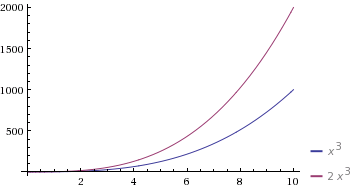
\includegraphics{graph}

The lines will never intersect.

40. Verify the $3x+1$ conjecture for these integers:

16, 8, 4, 2, 1

11, 34, 17, 52, 26, 13, 40, 20, 10, 5, 16, 8, 4, 2, 1

35, 106, 53, 160, 80, 40, 20, 10, 5, 16, 8, 4, 2, 1

113, 340, 170, 85, 256, 128, 64, 32, 16, 8, 4, 2, 1
\end{document}
